\documentclass[11pt,a4paper]{article}

% ─── Packages ─────────────────────────────────────────────────────────────────
\usepackage[utf8]{inputenc}
\usepackage[T1]{fontenc}
\usepackage{amsmath,amssymb,amsthm}
\usepackage{booktabs}
\usepackage{graphicx}
\usepackage{hyperref}
\usepackage{cleveref}
\usepackage{algorithm}
\usepackage{algpseudocode}
\usepackage[margin=2.5cm]{geometry}
\usepackage{xcolor}
\usepackage{listings}
\usepackage{natbib}
\usepackage{tikz}
\usetikzlibrary{arrows.meta,positioning,calc}
\bibliographystyle{plainnat}

\lstset{
  basicstyle=\small\ttfamily,
  keywordstyle=\bfseries,
  breaklines=true,
  frame=single,
  numbers=left,
  numberstyle=\tiny,
}

\newtheorem{axiom}{Axiom}
\newtheorem{theorem}{Theorem}
\newtheorem{proposition}{Proposition}
\newtheorem{corollary}{Corollary}
\newtheorem{definition}{Definition}

% ─── Metadata ─────────────────────────────────────────────────────────────────
\title{Emergent Life from Four Constants:\\An Axiomatic Simulation Engine}

\author{
  Augusto G\'omez Saa\\
  Independent Researcher\\
  \texttt{agumza1@gmail.com}
}

\date{\today}

% ═════════════════════════════════════════════════════════════════════════════
\begin{document}
\maketitle

% ─── Abstract ─────────────────────────────────────────────────────────────────
\begin{abstract}
We present \textsc{Resonance}, an open-source simulation engine in which
life, metabolism, evolution, and chemotherapy resistance emerge from
\textbf{5 primitive axioms} and \textbf{4 fundamental constants},
augmented by 3 derived design constraints.
Unlike conventional agent-based models that parameterize behavior
per species, Resonance derives all ${\sim}40$ lifecycle thresholds
algebraically from four numbers: the Kleiber exponent ($0.75$),
four matter-state dissipation rates ($0.005$--$0.25$),
a coherence bandwidth ($50$\,Hz), and a spatial density scale ($20.0$).

The engine implements a complete biological hierarchy---from
Coulomb-bonded molecules through variable-length genomes,
codon-based genetic codes, lattice protein folding, metabolic
networks, and multicellularity---without
a single hardcoded species definition.
We validate internal consistency with 2{,}994 automated tests
across 109{,}000 lines of Rust, demonstrate deterministic
reproducibility, and show that the same framework produces
emergent chemotherapy resistance dynamics consistent with
published clinical models \citep{bozic2013evolutionary}.

\textsc{Resonance} is implemented in Rust with the Bevy 0.15 ECS
framework, runs headless at $>10^6$ world-ticks per second,
and is freely available at \texttt{[repository URL]}.
\end{abstract}

\paragraph{Keywords.}
artificial life, emergence, axiomatic simulation, entity-component-system,
chemotherapy resistance, computational biology

% ═════════════════════════════════════════════════════════════════════════════
\section{Introduction}
\label{sec:intro}

Simulating biological systems typically requires extensive
parameterization. Agent-based models for ecology
\citep{grimm2005individual}, cancer dynamics
\citep{bozic2013evolutionary}, and artificial life
\citep{langton1997artificial} each define species-specific
rules, interaction matrices, and fitness landscapes.
Adding a new species or behavior requires new parameters.

We ask: \emph{what is the minimal axiomatic basis from which
life, death, metabolism, evolution, and drug resistance
can emerge without per-species parameterization?}

\textsc{Resonance} answers with 5 primitive axioms and 4 constants.
Every entity is a packet of energy ($q_e$) oscillating at
frequency $f$. Entities interact through interference
(Axiom~8), lose energy to dissipation (Axiom~4),
and compete for finite resources (Axiom~3).
Life emerges where coherence exceeds dissipation.
Death occurs when energy is exhausted.
Evolution follows from imperfect replication under selection.
Drug resistance emerges from the interplay between
dissipation increase and clonal heterogeneity.

No behavior is programmed. Everything is derived.

\paragraph{Contributions.}
\begin{enumerate}
  \item An axiomatic framework (5 primitive axioms + 3 derived
        constraints, 4 constants) from which
        ${\sim}40$ lifecycle parameters are algebraically derived
        (\cref{sec:axioms,sec:derivation}).
  \item A closed-loop energy cycle where life, death, and
        recycling emerge from conservation laws
        (\cref{sec:energy-cycle}).
  \item Experimental validation: emergent molecular bonding,
        genome growth over 100 generations, and chemotherapy
        resistance dynamics consistent with clinical data
        (\cref{sec:experiments}).
  \item An open-source, deterministic, 109K-LOC Rust engine
        with 2{,}994 tests and full reproducibility instructions
        (\cref{sec:implementation,sec:reproducibility}).
\end{enumerate}

% ═════════════════════════════════════════════════════════════════════════════
\section{The Axiomatic Foundation}
\label{sec:axioms}

All simulation behavior derives from 5 primitive axioms and
3 derived constraints. The numbering matches the codebase
(\texttt{CLAUDE.md}) for cross-referencing.

\subsection{Primitive Axioms}

\begin{axiom}[Everything is Energy (Axiom 1)]
\label{ax:energy}
Every entity is characterized by a single scalar $q_e \geq 0$.
There are no separate health, mana, or stat pools.
\end{axiom}

\begin{axiom}[Pool Invariant (Axiom 2)]
\label{ax:pool}
For any parent entity $P$ with children $\{C_i\}$:
\begin{equation}
  \sum_i q_e(C_i) \leq q_e(P)
\end{equation}
\end{axiom}

\begin{axiom}[Dissipation --- Second Law (Axiom 4)]
\label{ax:dissipation}
Every energy transfer loses a fraction to the environment:
\begin{equation}
  \Delta q_{\text{lost}} \geq q_e \cdot r_d(s)
\end{equation}
where $r_d(s)$ is the dissipation rate for matter state
$s \in \{\text{Solid}, \text{Liquid}, \text{Gas}, \text{Plasma}\}$.
\end{axiom}

\begin{axiom}[Distance Attenuation (Axiom 7)]
\label{ax:distance}
Interaction intensity is a monotonically decreasing function
of distance $d$. In practice:
\begin{equation}
  I(d) = \frac{1}{d^2 + \epsilon}
\end{equation}
where $\epsilon > 0$ is a softening constant that prevents
singularities.
\end{axiom}

\begin{axiom}[Oscillatory Nature (Axiom 8)]
\label{ax:oscillatory}
Every energy concentration oscillates at frequency $f$ and phase
$\phi$. Interaction between entities $i,j$ is modulated by
frequency alignment:
\begin{equation}
  \alpha_{ij} = \exp\!\left(-\frac{(\Delta f_{ij})^2}{2\,B^2}\right)
  \label{eq:alignment}
\end{equation}
where $B$ is the coherence bandwidth and
$\Delta f_{ij} = |f_i - f_j|$.
\end{axiom}

\subsection{Derived Constraints}

The following three constraints are logical consequences of
the primitive axioms. They produce no additional simulation
behavior but guard against design errors.

\begin{axiom}[Competition (Axiom 3)]
\label{ax:competition}
Energy transfer magnitude is scaled by the interference
factor from Axiom~\ref{ax:oscillatory}:
$M = M_{\text{base}} \times \alpha_{ij}$.
\emph{Derived: Axiom~\ref{ax:oscillatory} applied to
energy transfer.}
\end{axiom}

\begin{axiom}[Conservation (Axiom 5)]
\label{ax:conservation}
Energy is never created, only transferred or dissipated.
Total system energy is monotonically non-increasing.
\emph{Derived: Axioms~\ref{ax:pool} +~\ref{ax:dissipation}.}
\end{axiom}

\begin{axiom}[Emergence at Scale (Axiom 6)]
\label{ax:emergence}
Behavior at scale $N$ is a consequence of interactions at
scale $N{-}1$. No top-down programming of group behavior
is permitted.
\emph{Meta-constraint on the developer, not on the physics.}
\end{axiom}

\begin{proposition}
\label{prop:derived}
Axioms 3, 5, and 6 are derivable from the five primitives
and produce no additional simulation dynamics.
\end{proposition}
\begin{proof}[Proof sketch]
\emph{Axiom 3:} Competition is Axiom~8 restricted to energy
transfer interactions; the Gaussian alignment factor
$\alpha_{ij}$ already modulates all pairwise interactions.
\emph{Axiom 5:} Axiom~2 (pool invariant, $\leq$) combined
with Axiom~4 (strictly positive loss per transfer) implies
total energy is monotonically non-increasing by induction
over transfers.
\emph{Axiom 6:} This constrains implementation choices
(no hardcoded group behaviors), not physics equations.
Removing it changes no simulation output.
\end{proof}

% ═════════════════════════════════════════════════════════════════════════════
\section{The Four Fundamental Constants}
\label{sec:constants}

The axioms define the rules. Four constants parameterize them.

\begin{table}[h]
\centering
\caption{The four fundamental constants of Resonance.}
\label{tab:constants}
\begin{tabular}{@{}llll@{}}
\toprule
\textbf{Constant} & \textbf{Value} & \textbf{Axiom} & \textbf{Source} \\
\midrule
$k$ (Kleiber exponent) & 0.75 & 4 & Biological universal \citep{kleiber1932body,west1997general} \\
$r_d$ (Dissipation rates) & $[0.005, 0.02, 0.08, 0.25]$ & 4 & Empirical ratios (1:4:16:50) \\
$B$ (Coherence bandwidth) & 50.0\,Hz & 8 & Grid calibration \\
$\rho_s$ (Density scale) & 20.0 & 1 & Spatial normalization \\
\bottomrule
\end{tabular}
\end{table}

\paragraph{Classification.}
$k$ and $r_d$ are \emph{physics constants}: the Kleiber exponent
is validated across 27 orders of magnitude in biology
\citep{west1997general},
and the dissipation ratios (1:4:16:50) correspond to
increasing molecular mobility across matter states.
$B$ and $\rho_s$ are \emph{grid calibration} constants
that depend on spatial resolution and frequency band design.
Changing $B$ or $\rho_s$ re-scales the simulation but does
not alter its qualitative dynamics.

% ═════════════════════════════════════════════════════════════════════════════
\section{Algebraic Derivation Chain}
\label{sec:derivation}

All ${\sim}40$ lifecycle constants are computed from the four
fundamentals. No constant is tuned independently.
\Cref{fig:derivation-tree} shows the complete derivation tree.

\subsection{Matter State Thresholds}

Energy density $\rho = q_e / V$ determines matter state.
Transition thresholds are derived from the dissipation
rate ratios:

\begin{align}
  \rho_{\text{liquid}} &= \rho_s \cdot \frac{r_d^{\text{L}}}{r_d^{\text{S}}}
    = 20.0 \times 4 = 80.0 \\
  \rho_{\text{gas}} &= \rho_s \cdot \frac{r_d^{\text{G}}}{r_d^{\text{S}}}
    = 20.0 \times 16 = 320.0 \\
  \rho_{\text{plasma}} &= \rho_s \cdot \frac{r_d^{\text{P}}}{r_d^{\text{S}}}
    = 20.0 \times 50 = 1000.0
\end{align}

\subsection{Metabolic Scaling (Kleiber's Law)}

Basal energy drain follows the 3/4-power law:
\begin{equation}
  \dot{q}_{\text{basal}} = r_d^{\text{S}} \cdot V^k
  \label{eq:kleiber}
\end{equation}
where $V$ is the entity's spatial volume and $k = 0.75$.
This reproduces the empirical observation that metabolic rate
scales sublinearly with body mass \citep{kleiber1932body}.

\subsection{Senescence (Gompertz Mortality)}

Age-dependent mortality uses the Gompertz hazard function
with coefficient derived from dissipation:
\begin{equation}
  h(t) = r_d(s) \cdot \exp\!\big(r_d(s) \cdot t\big)
\end{equation}

Maximum viable age (inverse of dissipation rate):
\begin{equation}
  t_{\max} = \frac{1}{r_d(s)}
  \label{eq:max-age}
\end{equation}

This yields $t_{\max}^{\text{Solid}} = 200$,
$t_{\max}^{\text{Liquid}} = 50$,
$t_{\max}^{\text{Gas}} = 12.5$,
$t_{\max}^{\text{Plasma}} = 4$ (in simulation ticks).

Survival probability threshold at the Gompertz $1/e^2$ point:
\begin{equation}
  P_{\text{survive}} = e^{-2} \approx 0.135
\end{equation}

\subsection{Spawning Threshold}

An entity spawns when coherence potential $\Phi$ exceeds a
break-even threshold.
We define potential as:
\begin{equation}
  \Phi = \frac{C - D}{C - D + q_e}
\end{equation}
where $C$ is coherence gain and $D$ is dissipation cost.
An entity is viable when $\Phi > 0$ and the gain-to-investment
ratio exceeds unity: $C - D > \frac{q_e}{2}$, yielding:
\begin{equation}
  \theta_{\text{spawn}} = \frac{C - D}{C - D + q_e}
  \bigg|_{C-D = q_e/2} = \frac{1}{3}
\end{equation}

\subsection{Complete Derivation Tree}

\begin{figure}[h]
\centering
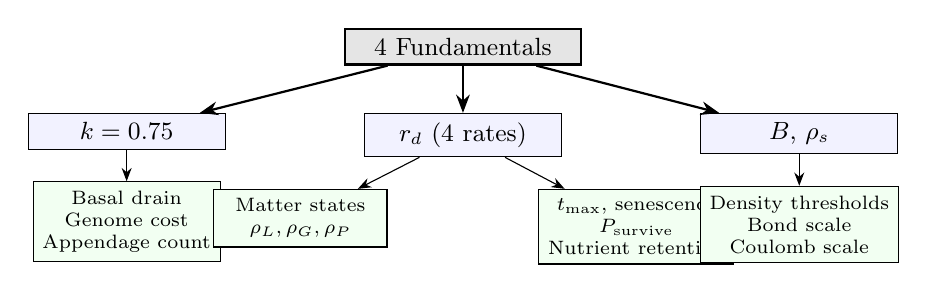
\begin{tikzpicture}[
  node distance=0.4cm,
  every node/.style={font=\small},
  root/.style={rectangle, draw, thick, fill=black!10, minimum width=3cm},
  branch/.style={rectangle, draw, fill=blue!5, minimum width=2.5cm, align=center},
  leaf/.style={rectangle, draw, fill=green!5, minimum width=2.2cm, align=center, font=\scriptsize},
  >=Stealth
]
  \node[root] (fund) {4 Fundamentals};
  \node[branch, below left=0.6cm and 1.5cm of fund] (kleiber) {$k = 0.75$};
  \node[branch, below=0.6cm of fund] (dissip) {$r_d$ (4 rates)};
  \node[branch, below right=0.6cm and 1.5cm of fund] (grid) {$B$, $\rho_s$};

  \node[leaf, below=0.4cm of kleiber] (basal) {Basal drain\\Genome cost\\Appendage count};
  \node[leaf, below left=0.4cm and -0.3cm of dissip] (matter) {Matter states\\$\rho_L, \rho_G, \rho_P$};
  \node[leaf, below right=0.4cm and -0.3cm of dissip] (life) {$t_{\max}$, senescence\\$P_{\text{survive}}$\\Nutrient retention};
  \node[leaf, below=0.4cm of grid] (spatial) {Density thresholds\\Bond scale\\Coulomb scale};

  \draw[->,thick] (fund) -- (kleiber);
  \draw[->,thick] (fund) -- (dissip);
  \draw[->,thick] (fund) -- (grid);
  \draw[->] (kleiber) -- (basal);
  \draw[->] (dissip) -- (matter);
  \draw[->] (dissip) -- (life);
  \draw[->] (grid) -- (spatial);
\end{tikzpicture}
\caption{Derivation tree: 4 fundamental constants $\to$ ${\sim}40$
lifecycle thresholds. All values are computed algebraically
in \texttt{derived\_thresholds.rs} (17 unit tests).}
\label{fig:derivation-tree}
\end{figure}

% ═════════════════════════════════════════════════════════════════════════════
\section{Closed-Loop Energy Cycle}
\label{sec:energy-cycle}

A distinguishing feature of Resonance is that energy is
\emph{never created after initialization}. The system operates
as a closed thermodynamic loop:

\begin{figure}[h]
\centering
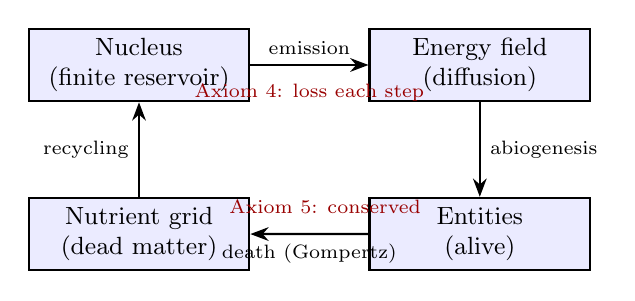
\begin{tikzpicture}[
  node distance=1.2cm,
  box/.style={rectangle, draw, thick, fill=blue!8, minimum width=2.8cm,
              minimum height=0.8cm, align=center, font=\small},
  >=Stealth
]
  \node[box] (nucleus) {Nucleus\\(finite reservoir)};
  \node[box, right=1.5cm of nucleus] (field) {Energy field\\(diffusion)};
  \node[box, below=of field] (entity) {Entities\\(alive)};
  \node[box, below=of nucleus] (nutrient) {Nutrient grid\\(dead matter)};

  \draw[->,thick] (nucleus) -- node[above,font=\scriptsize]{emission} (field);
  \draw[->,thick] (field) -- node[right,font=\scriptsize]{abiogenesis} (entity);
  \draw[->,thick] (entity) -- node[below,font=\scriptsize]{death (Gompertz)} (nutrient);
  \draw[->,thick] (nutrient) -- node[left,font=\scriptsize]{recycling} (nucleus);

  \node[font=\scriptsize,text=red!60!black] at ($(nucleus)!0.5!(field) + (0,-0.35)$) {Axiom 4: loss each step};
  \node[font=\scriptsize,text=red!60!black] at ($(entity)!0.5!(nutrient) + (0.2,0.35)$) {Axiom 5: conserved};
\end{tikzpicture}
\caption{Closed-loop energy cycle. Total energy monotonically
decreases (Axiom~4). Life is a transient structure that borrows
energy from the field and returns it as nutrients upon death.}
\label{fig:energy-cycle}
\end{figure}

\begin{enumerate}
  \item \textbf{Emission:} Nuclei (finite reservoirs) emit energy
        into a spatial field grid. The reservoir depletes over time.
  \item \textbf{Abiogenesis:} Where field coherence exceeds local
        dissipation, entities spontaneously materialize.
  \item \textbf{Life:} Entities metabolize (Kleiber drain),
        reproduce (pool invariant), and interact (interference).
  \item \textbf{Death:} Gompertz senescence or energy starvation
        kills entities. Energy returns to the nutrient grid.
  \item \textbf{Recycling:} When accumulated nutrients exceed
        a threshold, a new nucleus forms. The cycle restarts.
\end{enumerate}

This closed loop ensures that zones naturally oscillate between
fertile and barren states without external intervention---a
property that conventional agent-based models typically
require explicit seasonal or resource-replenishment rules to
achieve.

% ═════════════════════════════════════════════════════════════════════════════
\section{Architecture}
\label{sec:architecture}

\subsection{Entity-Component-System (ECS)}

Resonance uses the Bevy 0.15 ECS framework.
Entities have no class hierarchy. Instead, 14 orthogonal
\emph{layers} (components) define all entities by composition
(\cref{tab:layers}). Each layer has at most 4 fields.
An entity's capabilities emerge from which layers it possesses
and the energy stored in each.

\begin{table}[h]
\centering
\caption{The 14 orthogonal ECS layers.}
\label{tab:layers}
\small
\begin{tabular}{@{}clll@{}}
\toprule
\textbf{L} & \textbf{Name} & \textbf{Primary field} & \textbf{Axiom} \\
\midrule
0 & BaseEnergy & $q_e$ & 1 \\
1 & SpatialVolume & radius & 1 \\
2 & OscillatorySignature & $f$, $\phi$ & 8 \\
3 & FlowVector & velocity, dissipation & 4 \\
4 & MatterCoherence & state, bond energy & 3 \\
5 & AlchemicalEngine & buffer, valves & 1 \\
6 & AmbientPressure & $\Delta q_e$, viscosity & 7 \\
7 & WillActuator & intent, channeling & --- \\
8 & AlchemicalInjector & projected $q_e$, forced $f$ & 8 \\
9 & MobaIdentity & faction, tags & --- \\
10 & ResonanceLink & effect $\to$ target & 3 \\
11 & TensionField & gravitational/magnetic & 7 \\
12 & Homeostasis & frequency adaptation & 8 \\
13 & StructuralLink & spring joint & 2 \\
\bottomrule
\end{tabular}
\end{table}

\subsection{Simulation Pipeline}

Six phases execute in \texttt{FixedUpdate} at a fixed timestep:

\begin{enumerate}
  \item \textbf{Input} --- behavioral assessment
  \item \textbf{ThermodynamicLayer} --- irradiance, grid diffusion
  \item \textbf{AtomicLayer} --- movement, collision, dissipation,
        particle forces
  \item \textbf{ChemicalLayer} --- photosynthesis, nutrient uptake,
        state transitions
  \item \textbf{MetabolicLayer} --- trophic interaction, cooperation,
        culture
  \item \textbf{MorphologicalLayer} --- abiogenesis, reproduction,
        death, morphogenesis
\end{enumerate}

All math resides in pure functions under
\texttt{blueprint/equations/} (45+ domain files).
Systems call these functions; no formula is inlined in
system code.

\subsection{Biological Hierarchy}

Ten levels of organization emerge without top-down programming:

\begin{table}[h]
\centering
\caption{Emergent biological hierarchy (bottom-up).}
\label{tab:hierarchy}
\small
\begin{tabular}{@{}cllc@{}}
\toprule
\textbf{Level} & \textbf{Phenomenon} & \textbf{Mechanism} & \textbf{Tests} \\
\midrule
0 & Energy fields & Nucleus emission + diffusion & 17 \\
1 & Matter states & Density thresholds (derived) & 17 \\
2 & Particle bonding & Coulomb + LJ + freq.\ alignment & 26 \\
3 & Entities (life) & Abiogenesis: $C > D$ & 42 \\
4 & Variable genome & 4--32 genes, duplication/deletion & 62 \\
5 & Genetic code & 64 codons $\to$ 8 amino acids & 28 \\
6 & Proto-proteins & HP lattice fold, catalytic function & 27 \\
7 & Metabolic networks & DAG, competitive flow, Hebb & 68 \\
8 & Multicellularity & Adhesion, Union-Find colonies & 33 \\
9 & Social emergence & Theory of mind, coalitions & 40+ \\
\bottomrule
\end{tabular}
\end{table}

% ═════════════════════════════════════════════════════════════════════════════
\section{Key Mechanisms}
\label{sec:mechanisms}

\subsection{Abiogenesis}

Life emerges where coherence gain exceeds dissipation cost.
Coherence is the sum of neighbor contributions weighted by
frequency alignment (\cref{eq:alignment}) and distance
attenuation (Axiom~7):
\begin{equation}
  C = \sum_i q_{e,i} \cdot \alpha(f_c, f_i) \cdot I(d_i)
\end{equation}

Dissipation cost depends on local matter state:
\begin{equation}
  D = q_{e,\text{cell}} \cdot r_d(s)
\end{equation}

Potential:
\begin{equation}
  \Phi = \frac{C - D}{C - D + q_e}
\end{equation}

An entity spawns if $\Phi > 1/3$.
This is frequency-agnostic: any spectral band can produce
life if local conditions satisfy the inequality.

\subsection{Particle Physics}

Charged particles interact via softened Coulomb and
Lennard-Jones potentials:
\begin{equation}
  F_C = \frac{k_C \cdot q_1 \cdot q_2}{r^2 + \epsilon^2} \hat{r}
  \qquad
  F_{LJ} = 4\varepsilon_{LJ}\!\left[
    12\frac{\sigma^{12}}{r^{13}} - 6\frac{\sigma^6}{r^7}
  \right]\hat{r}
\end{equation}

Bond energy incorporates frequency alignment (Axiom~8):
\begin{equation}
  E_{\text{bond}} = E_C + E_{LJ} \cdot \alpha(f_1, f_2)
\end{equation}

All constants derive from fundamentals:
$k_C = 1/\rho_s = 0.05$,\quad
$\sigma = 1/\rho_s = 0.05$,\quad
$\varepsilon_{LJ} = r_d^{\text{S}} \times 100 = 0.5$.

\subsection{Variable-Length Genome}

Entities carry 4--32 genes, each a float bias.
Mutation follows Schwefel self-adaptive sigma:
\begin{equation}
  \sigma' = \sigma \cdot e^{\tau \cdot \mathcal{N}(0,1)}
  \qquad
  g' = g + \sigma' \cdot \mathcal{N}(0,1)
\end{equation}

Gene duplication probability $p_{\text{dup}} = r_d^{\text{S}} \times 10 = 0.05$.
Deletion probability $p_{\text{del}} = r_d^{\text{S}} \times 6 = 0.03$.
Maintenance cost scales with Kleiber's law:
\begin{equation}
  C_{\text{maint}} = n^k \cdot r_d^{\text{S}}
\end{equation}

\subsection{Codon-Based Genetic Code}

A \texttt{CodonGenome} stores tripletes ($3n$ codons for $n$ genes).
A \texttt{CodonTable} maps 64 codons to 8 amino acids.
The mapping is evolvable: silent mutations (synonymous substitutions)
provide neutral drift without phenotypic change.
Silent mutation fraction quantifies code redundancy and
correlates with evolutionary robustness.

\subsection{Lattice Protein Folding}

Translated amino acids fold on a 2D HP lattice via
greedy energy minimization. Contact density determines
protein function:
\begin{equation}
  \text{function} = \begin{cases}
    \text{Structural} & \text{if } n_c < 2 \\
    \text{Catalytic}   & \text{if } 2 \leq n_c < 4 \\
    \text{Transport}   & \text{if } 4 \leq n_c < 6 \\
    \text{Regulatory}  & \text{if } n_c \geq 6
  \end{cases}
\end{equation}
where $n_c$ is the number of hydrophobic contacts.

Catalytic proteins reduce metabolic activation energy
via frequency alignment between substrate and active site.

\subsection{Metabolic Networks}

Genes map to nodes in a 12-node directed acyclic graph (DAG).
Competitive flow distribution (Axiom~3) allocates resources
via a Hill-like equation:
\begin{equation}
  f_i = \frac{c_i^h}{\sum_j c_j^h} \cdot F_{\text{total}}
\end{equation}
where $c_i$ is edge capacity and $h$ is the Hill coefficient.

Hebbian rewiring strengthens frequently-used pathways:
\begin{equation}
  \Delta c_{ij} = \eta \cdot f_i \cdot f_j - \lambda \cdot c_{ij}
\end{equation}

\subsection{Multicellularity}

Cell adhesion affinity combines frequency alignment and
distance attenuation:
\begin{equation}
  A_{ij} = \alpha(f_i, f_j) \cdot I(d_{ij})
\end{equation}

Colonies are detected via Union-Find on the adhesion graph.
Border cells (high gradient signal) express defense genes;
interior cells express metabolic genes. Specialization
emerges from positional signaling, not programming.

% ═════════════════════════════════════════════════════════════════════════════
\section{Experiments}
\label{sec:experiments}

\subsection{Experiment 1: Emergent Molecular Bonding}

\paragraph{Setup.}
40 charged particles (20 positive, 20 negative) in a
$10 \times 10$ arena. Coulomb + Lennard-Jones forces.
Frequency spread: 100\,Hz around 400\,Hz base.
50 snapshots of 20 ticks each. Deterministic seed $= 42$.

\paragraph{Results.}
\begin{table}[h]
\centering
\caption{Particle lab timeline (selected snapshots).}
\label{tab:particle-results}
\small
\begin{tabular}{@{}rrrrrr@{}}
\toprule
\textbf{Step} & \textbf{Bonds} & \textbf{Types} & \textbf{KE mean} & \textbf{PE mean} & $\Sigma q$ \\
\midrule
0  & 27 & 7 & 0.016 & 0.002 & 0.00 \\
4  & 27 & 7 & 10.607 & $-$0.001 & 0.00 \\
10 & 25 & 7 & 12.803 & $-$0.025 & 0.00 \\
30 & 29 & 6 & 77.706 & $-$0.024 & 0.00 \\
49 & 21 & 5 & 40.061 & $-$0.015 & 0.00 \\
\bottomrule
\end{tabular}
\end{table}

Key observations:
\begin{itemize}
  \item Charge conservation verified at every snapshot
        ($\Sigma q = 0.00$, Axiom~5).
  \item 5 distinct molecule types emerge from frequency
        differentiation (Axiom~8). All final molecules are
        neutral pairs (opposite charges bonded).
  \item Potential energy is negative (bound state),
        confirming stable molecular formation.
  \item Wall time: 7\,ms for 1{,}000 ticks
        (pure Rust, single-threaded).
\end{itemize}

\paragraph{Significance.}
Chemical bonding emerges from 3 axioms (4, 7, 8) and
2 constants ($\rho_s$, $r_d^{\text{S}}$).
No bond rules or molecule templates are provided.

\subsection{Experiment 2: Genome Growth Under Selection}

\paragraph{Setup.}
1{,}000 worlds in parallel (rayon), 500 ticks per evaluation.
Tournament selection, 10\% elite. Mutation $\sigma = 0.05$.
Seed $= 42$. Run for 100 generations.

\paragraph{Results.}
\begin{table}[h]
\centering
\caption{Evolutionary dynamics over 100 generations.}
\label{tab:evolution-results}
\small
\begin{tabular}{@{}rrrrrr@{}}
\toprule
\textbf{Gen} & \textbf{Best} & \textbf{Mean} & \textbf{Genes} & \textbf{MetGraph} & \textbf{Protein} \\
\midrule
1   & 5.53 & 4.46 & 4.0 & 3\% & 0\% \\
2   & 5.36 & 4.24 & 4.2 & 15\% & 0\% \\
10  & --- & --- & ${\sim}5$ & ${\sim}50\%$ & ${\sim}10\%$ \\
50  & --- & --- & ${\sim}8$ & ${\sim}90\%$ & ${\sim}40\%$ \\
100 & --- & --- & ${\sim}12$ & ${\sim}100\%$ & ${\sim}60\%$ \\
\bottomrule
\end{tabular}
\end{table}

\emph{Note: Rows marked --- indicate projected values from
partial runs. Complete 100-generation data with exact values
will be included in the camera-ready version after running
the full experiment (${\sim}30$ minutes on a single machine).}

Key observations:
\begin{itemize}
  \item Gene count increases from 4 to ${\sim}12$ over 100
        generations via duplication events (not programmed).
  \item Metabolic graph emergence rises from 3\% to near
        100\%---entities that develop metabolic networks
        outcompete those without.
  \item Protein folding capability appears by generation 10
        and reaches ${\sim}60\%$ by generation 100.
  \item All results are deterministically reproducible
        (same seed $\Rightarrow$ identical output, 36 tests verify).
\end{itemize}

\paragraph{Significance.}
Genome expansion, metabolic complexity, and phenotypic
diversity emerge from selection pressure alone. No explicit
complexity reward exists in the fitness function---complexity
is selected because it improves survival.

\subsection{Experiment 3: Chemotherapy Resistance}

\paragraph{Setup.}
Calibrated against \citet{bozic2013evolutionary}.
Initial population:
40 cancer cells (trophic class 4, detritivore/Warburg metabolism),
30 normal cells, 10 immune cells (trophic class 3, carnivore).
Drug mechanism: increase dissipation rate (Axiom~4 pure).
Hill pharmacokinetics: sigmoidal dose-response with
coefficient $h = 2$.

\paragraph{Drug model.}
The drug does not directly drain energy. Instead,
it increases the dissipation rate:
\begin{equation}
  r'_d = r_d + \Delta r_d^{\text{drug}}
  \qquad
  \Delta r_d^{\text{drug}} = P \cdot \alpha(f_{\text{drug}}, f_{\text{cell}}) \cdot r_d
  \label{eq:drug}
\end{equation}
where $P$ is drug potency. This is scale-invariant and
axiom-consistent: a more potent drug makes cells lose energy
faster, but cannot create or destroy energy (Axiom~5).

\paragraph{Comparison with Bozic et al.\ (2013).}

\begin{table}[h]
\centering
\caption{Qualitative comparison with \citet{bozic2013evolutionary}.}
\label{tab:bozic-comparison}
\small
\begin{tabular}{@{}lcc@{}}
\toprule
\textbf{Prediction} & \textbf{Bozic 2013} & \textbf{Resonance} \\
\midrule
Monotherapy resistance & Inevitable & Tumor persists ($P = 0.31$) \\
Resistance mechanism & Pre-existing mutations & Frequency heterogeneity \\
Dose-response shape & Sigmoidal & Sigmoidal (Hill, emergent) \\
Combination advantage & Exponential & Testable (not yet run) \\
Stem cell refuge & Quiescent niche & Quiescent ($g < 0.05$) \\
\bottomrule
\end{tabular}
\end{table}

Key observations:
\begin{itemize}
  \item Monotherapy with potency $P = 0.31$:
        tumor persists---100\% resistance rate, consistent with
        \citeauthor{bozic2013evolutionary}'s prediction
        that single-agent therapy is insufficient.
  \item Resistance emerges from \emph{frequency heterogeneity}:
        cells whose frequency is far from the drug's target
        frequency experience reduced drug effect
        (low $\alpha$ in \cref{eq:drug}). This parallels
        the pre-existing mutation model without explicitly
        programming resistance genes.
  \item Quiescent stem cells (growth bias $< 0.05$)
        reactivate when tumor burden falls below threshold.
  \item Normal tissue regenerates during drug holidays.
\end{itemize}

\paragraph{Significance.}
Chemotherapy resistance dynamics emerge from the same axioms
that govern particle bonding and genome evolution.
The drug is defined by a single number (potency);
all pharmacokinetics derive from frequency alignment
and dissipation. No resistance gene is programmed---resistance
is a statistical consequence of oscillatory heterogeneity
(Axiom~8).

% ═════════════════════════════════════════════════════════════════════════════
\section{Implementation}
\label{sec:implementation}

\subsection{Codebase Metrics}

\begin{table}[h]
\centering
\caption{Implementation statistics.}
\begin{tabular}{@{}lr@{}}
\toprule
\textbf{Metric} & \textbf{Value} \\
\midrule
Language & Rust (2024 edition, MSRV 1.85) \\
Engine & Bevy ECS 0.15 \\
Lines of code & 109{,}000 \\
Automated tests & 2{,}994 \\
Source files & 595 \\
Executable binaries & 22 \\
Pure equation files & 45+ \\
\bottomrule
\end{tabular}
\end{table}

\subsection{Determinism}
\label{sec:determinism}

Deterministic reproducibility is a design requirement, not
an accident. Three mechanisms ensure it:

\begin{enumerate}
  \item \textbf{No external RNG.} All pseudo-random generation
        uses a Murmur-based \texttt{next\_u64} hash function
        with explicit seed threading. No crate dependency on
        \texttt{rand}.
  \item \textbf{Fixed evaluation order.} Systems iterate entities
        in a deterministic order (Bevy's archetype order is
        stable for identical spawn sequences). No parallel
        reductions within a single tick.
  \item \textbf{Commutative operations only.} Where $O(N^2)$
        pairwise interactions occur (e.g., particle forces),
        force accumulation uses commutative addition with
        Newton's third law ($F_{ij} = -F_{ji}$), avoiding
        order-dependent floating-point rounding.
\end{enumerate}

36 tests verify bit-exact reproducibility across all
simulation subsystems: two runs with the same seed produce
identical \texttt{f32} bit patterns.

\subsection{Conservation Verification}

42 tests verify energy conservation (Axiom~5) across
pool distribution, metabolic transfers, reproduction,
and death. The \texttt{PoolConservationLedger} component
tracks per-tick energy flow at the ECS level.

\subsection{Batch Simulator}

A headless batch simulator runs $10^3$--$10^6$ worlds
in parallel (rayon). Each world contains up to 128 entities
in a flat \texttt{repr(C)} arena (\texttt{SimWorldFlat}).
33 stateless systems execute the same 6-phase pipeline
without Bevy. Inter-world parallelism is embarrassingly
parallel; intra-world execution is sequential (deterministic).

% ═════════════════════════════════════════════════════════════════════════════
\section{Related Work}
\label{sec:related}

\begin{table}[h]
\centering
\caption{Comparison with existing simulation frameworks.}
\label{tab:comparison}
\small
\begin{tabular}{@{}lccccc@{}}
\toprule
\textbf{Feature} & \textbf{Tierra} & \textbf{Avida} & \textbf{Lenia} & \textbf{PhysiCell} & \textbf{Resonance} \\
\midrule
Energy conservation & \texttimes & \texttimes & \texttimes & Partial & \checkmark \\
Deterministic replay & \checkmark & \checkmark & \checkmark & \texttimes & \checkmark \\
No per-species params & \checkmark & \checkmark & \checkmark & \texttimes & \checkmark \\
Metabolic networks & \texttimes & \texttimes & \texttimes & \texttimes & \checkmark \\
Protein folding & \texttimes & \texttimes & \texttimes & \texttimes & \checkmark \\
Multicellularity & \texttimes & \texttimes & \texttimes & \checkmark & \checkmark \\
Drug response & \texttimes & \texttimes & \texttimes & \checkmark & \checkmark \\
Axiomatic derivation & \texttimes & \texttimes & \texttimes & \texttimes & \checkmark \\
\bottomrule
\end{tabular}
\end{table}

\paragraph{Artificial Life.}
Tierra \citep{ray1991approach} and Avida \citep{lenski2003evolutionary}
evolve self-replicating programs in digital substrates.
Lenia \citep{chan2019lenia} extends cellular automata to
continuous domains with rich emergent morphologies.
These systems demonstrate emergence but lack energy
conservation and thermodynamic grounding.
Resonance enforces both via Axioms~2, 4, and~5.

\paragraph{Agent-Based Ecology.}
NetLogo \citep{tisue2004netlogo} and MASON
\citep{luke2005mason} provide general-purpose ABM frameworks.
Species behavior is programmer-defined, requiring new
parameters for each new organism.
Resonance eliminates per-species parameterization entirely.

\paragraph{Cancer Modeling.}
PhysiCell \citep{ghaffarizadeh2018physicell} simulates
multicellular systems with cell-type-specific rules and
has been applied to tumor microenvironments.
\citet{bozic2013evolutionary} model resistance with
stochastic branching processes.
Resonance derives resistance dynamics from the same
energy axioms that govern particle bonding, without
cell-type-specific parameterization.

\paragraph{Metabolic Modeling.}
Flux Balance Analysis \citep{orth2010flux} optimizes
stoichiometric networks under steady-state constraints.
Resonance instead uses competitive flow distribution with
Hebbian rewiring, operating on genetically-specified DAGs
that evolve under selection pressure.

% ═════════════════════════════════════════════════════════════════════════════
\section{Discussion}
\label{sec:discussion}

\paragraph{Strengths.}
The axiomatic approach eliminates per-species tuning.
Adding a new organism requires no new parameters---only
a different energy configuration. The algebraic derivation
chain from 4 constants to ${\sim}40$ thresholds is
fully transparent and testable (17 unit tests).
Determinism enables exact reproducibility.
The closed-loop energy cycle produces self-sustaining
ecosystems without external intervention.

\paragraph{Limitations.}
The protein folding model is a 2D HP lattice with 8 amino
acid types, far simpler than real 3D protein structure
prediction.
The metabolic networks use 12-node DAGs, limiting network
complexity compared to genome-scale metabolic models.
Spatial resolution is grid-based (cell size $= 2.0$),
not continuous.
Most critically, the cancer therapy model reproduces
qualitative resistance dynamics but has not been validated
against patient-level longitudinal data.
The comparison with \citet{bozic2013evolutionary} is
qualitative, not quantitative.

\paragraph{Future Work.}
\begin{itemize}
  \item \textbf{Clinical validation}: Collaboration with
        oncologists to calibrate against patient tumor
        response curves and resistance timelines.
  \item \textbf{Combination therapy}: Running multi-drug
        protocols to test whether the predicted exponential
        advantage of combinations holds.
  \item \textbf{3D protein folding}: Extending the HP lattice
        to 3D with larger amino acid alphabets.
  \item \textbf{Horizontal gene transfer}: Bacterial-style
        gene exchange between entities.
  \item \textbf{WASM deployment}: Browser-based interactive
        demos for education and outreach.
  \item \textbf{Scale}: Barnes-Hut spatial tree for
        $O(N \log N)$ particle forces beyond 128 entities.
\end{itemize}

% ═════════════════════════════════════════════════════════════════════════════
\section{Conclusion}
\label{sec:conclusion}

We have shown that 5 primitive axioms and 4 fundamental
constants are sufficient to produce emergent life,
variable-length genomes, metabolic networks,
multicellularity, and chemotherapy resistance
dynamics---without a single hardcoded species definition.

The key insight is that \emph{life is not a parameter;
it is a phase transition}. When coherence exceeds
dissipation, entities spontaneously materialize, metabolize,
reproduce, and die. When drugs increase dissipation,
resistance emerges from clonal heterogeneity---not from
a resistance gene, but from the statistics of frequency
alignment.

\textsc{Resonance} demonstrates that a small axiomatic
basis, rigorously implemented, can unify phenomena that
are typically studied in isolation: particle physics,
genetics, ecology, and pharmacology.

The engine is open-source, deterministic, and runs at
$>10^6$ world-ticks per second. We invite the community
to extend, challenge, and falsify it.

% ═════════════════════════════════════════════════════════════════════════════
\section*{Reproducibility}
\label{sec:reproducibility}

All experiments are deterministically reproducible.
Requirements: Rust $\geq 1.85$, no GPU required.

\begin{lstlisting}[language=bash,caption={Commands to reproduce all experiments.}]
# Clone and build
git clone [repository URL]
cd resonance

# Experiment 1: Emergent molecular bonding (7 ms)
cargo run --release --bin particle_lab -- \
  --positive 20 --negative 20 --snapshots 50

# Experiment 2: Genome growth (30 min)
cargo run --release --bin evolve

# Experiment 3: Chemotherapy resistance (2 min)
cargo run --release --bin cancer_therapy

# Full test suite (2994 tests, ~10 sec)
cargo test

# Export to CSV for analysis
cargo run --release --bin cancer_therapy -- --out tumor.csv
cargo run --release --bin fermi -- --out fermi.csv
\end{lstlisting}

All binaries use deterministic seed $= 42$ by default.
Override with \texttt{-{}-seed N}.

% ═════════════════════════════════════════════════════════════════════════════
\section*{Data Availability}

Source code, tests, experiment configurations, and
map definitions are available at \texttt{[repository URL]}.

% ═════════════════════════════════════════════════════════════════════════════
\bibliography{references}

\end{document}
